\documentclass{report}
\usepackage{graphicx} % Required for inserting images
\usepackage{float}
\usepackage{hyperref}

\usepackage[italian]{babel}
\usepackage[italian]{cleveref}

\setcounter{tocdepth}{3}
\setcounter{secnumdepth}{3}

\title{
\normalsize{Corso di Sistemi Embedded e Internet of Things}\\
\Huge{Smart Waste Disposal System}\\
\vspace{0.75em}
\large{Progettazione e costruzione di un \textit{raccoglirifiuti intelligente} ed implementazione di una Macchina a Stati Finiti}
}
\author{Luca Ponseggi \and Jacopo Turchi \and Luca Venturini \and Federico Bagattoni}
\date{\today}

\begin{document}

\maketitle

\tableofcontents
\newpage
\section*{Introduzione}
\par{
L'obbiettivo del progetto è costruire e progettare un raccoglifiuti intelligente che permetta agli utenti di depositare rifiuti liquidi controllando la temperatura ed il livello di riempimento del contenitore, avvisando in caso di necessità gli addetti alla manutenzione.
}
\par{
Per lo sviluppo verrà utilizzata la piattaforma \textbf{Arduno Uno} e diversi sensori sia analogici che digitali.
}

\chapter{Architettura}
\par {
La soluzione proposta dal gruppo si fonda su un'architettura \textit{task-based}. Questo approccio si basa sull'idea che il comportamento di un sistema embedded possa essere suddiviso in una serie di compiti (\textit{tasks}), che vengono eseguiti in modo concorrente o pseudo-concorrente. La caratteristica fondamentale di questa architettura è la \textbf{modularità}: ogni task è rappresentato come un modulo indipendente, nel nostro caso strutturato in una coppia di file, un file header e il relativo file \texttt{.cpp}.
}
\par {
Tutti i task vengono gestiti da uno \textbf{scheduler}, che ha la responsabilità di eseguirli in sequenza, cercando di eseguirli nel più breve tempo possibile, creando l'illusione che vengano eseguiti contemporaneamente. Inoltre, il sistema adotta una Macchina a Stati Finiti (MSF), che determina le azioni da intraprendere per ciascun task, in base allo stato corrente del sistema.
}

\section{Task del sistema}

\par{
L'architettura prevede 6 tasks: 
}
\begin{itemize}
    \item {
    \textbf{Main task}: il task principale del sistema di gestione intelligente dei rifiuti (detto nella codebase \textbf{Smart Waste Disposal System}) che ne controlla il comportamento generale. Essa esegue un ciclo continuo (tick()), monitorando gli stati e coordinando le azioni tra vari componenti, come il rilevamento dell'utente, l'apertura del contenitore, la gestione dello smaltimento e la manutenzione.
    \begin{figure}[H]
        \centering
        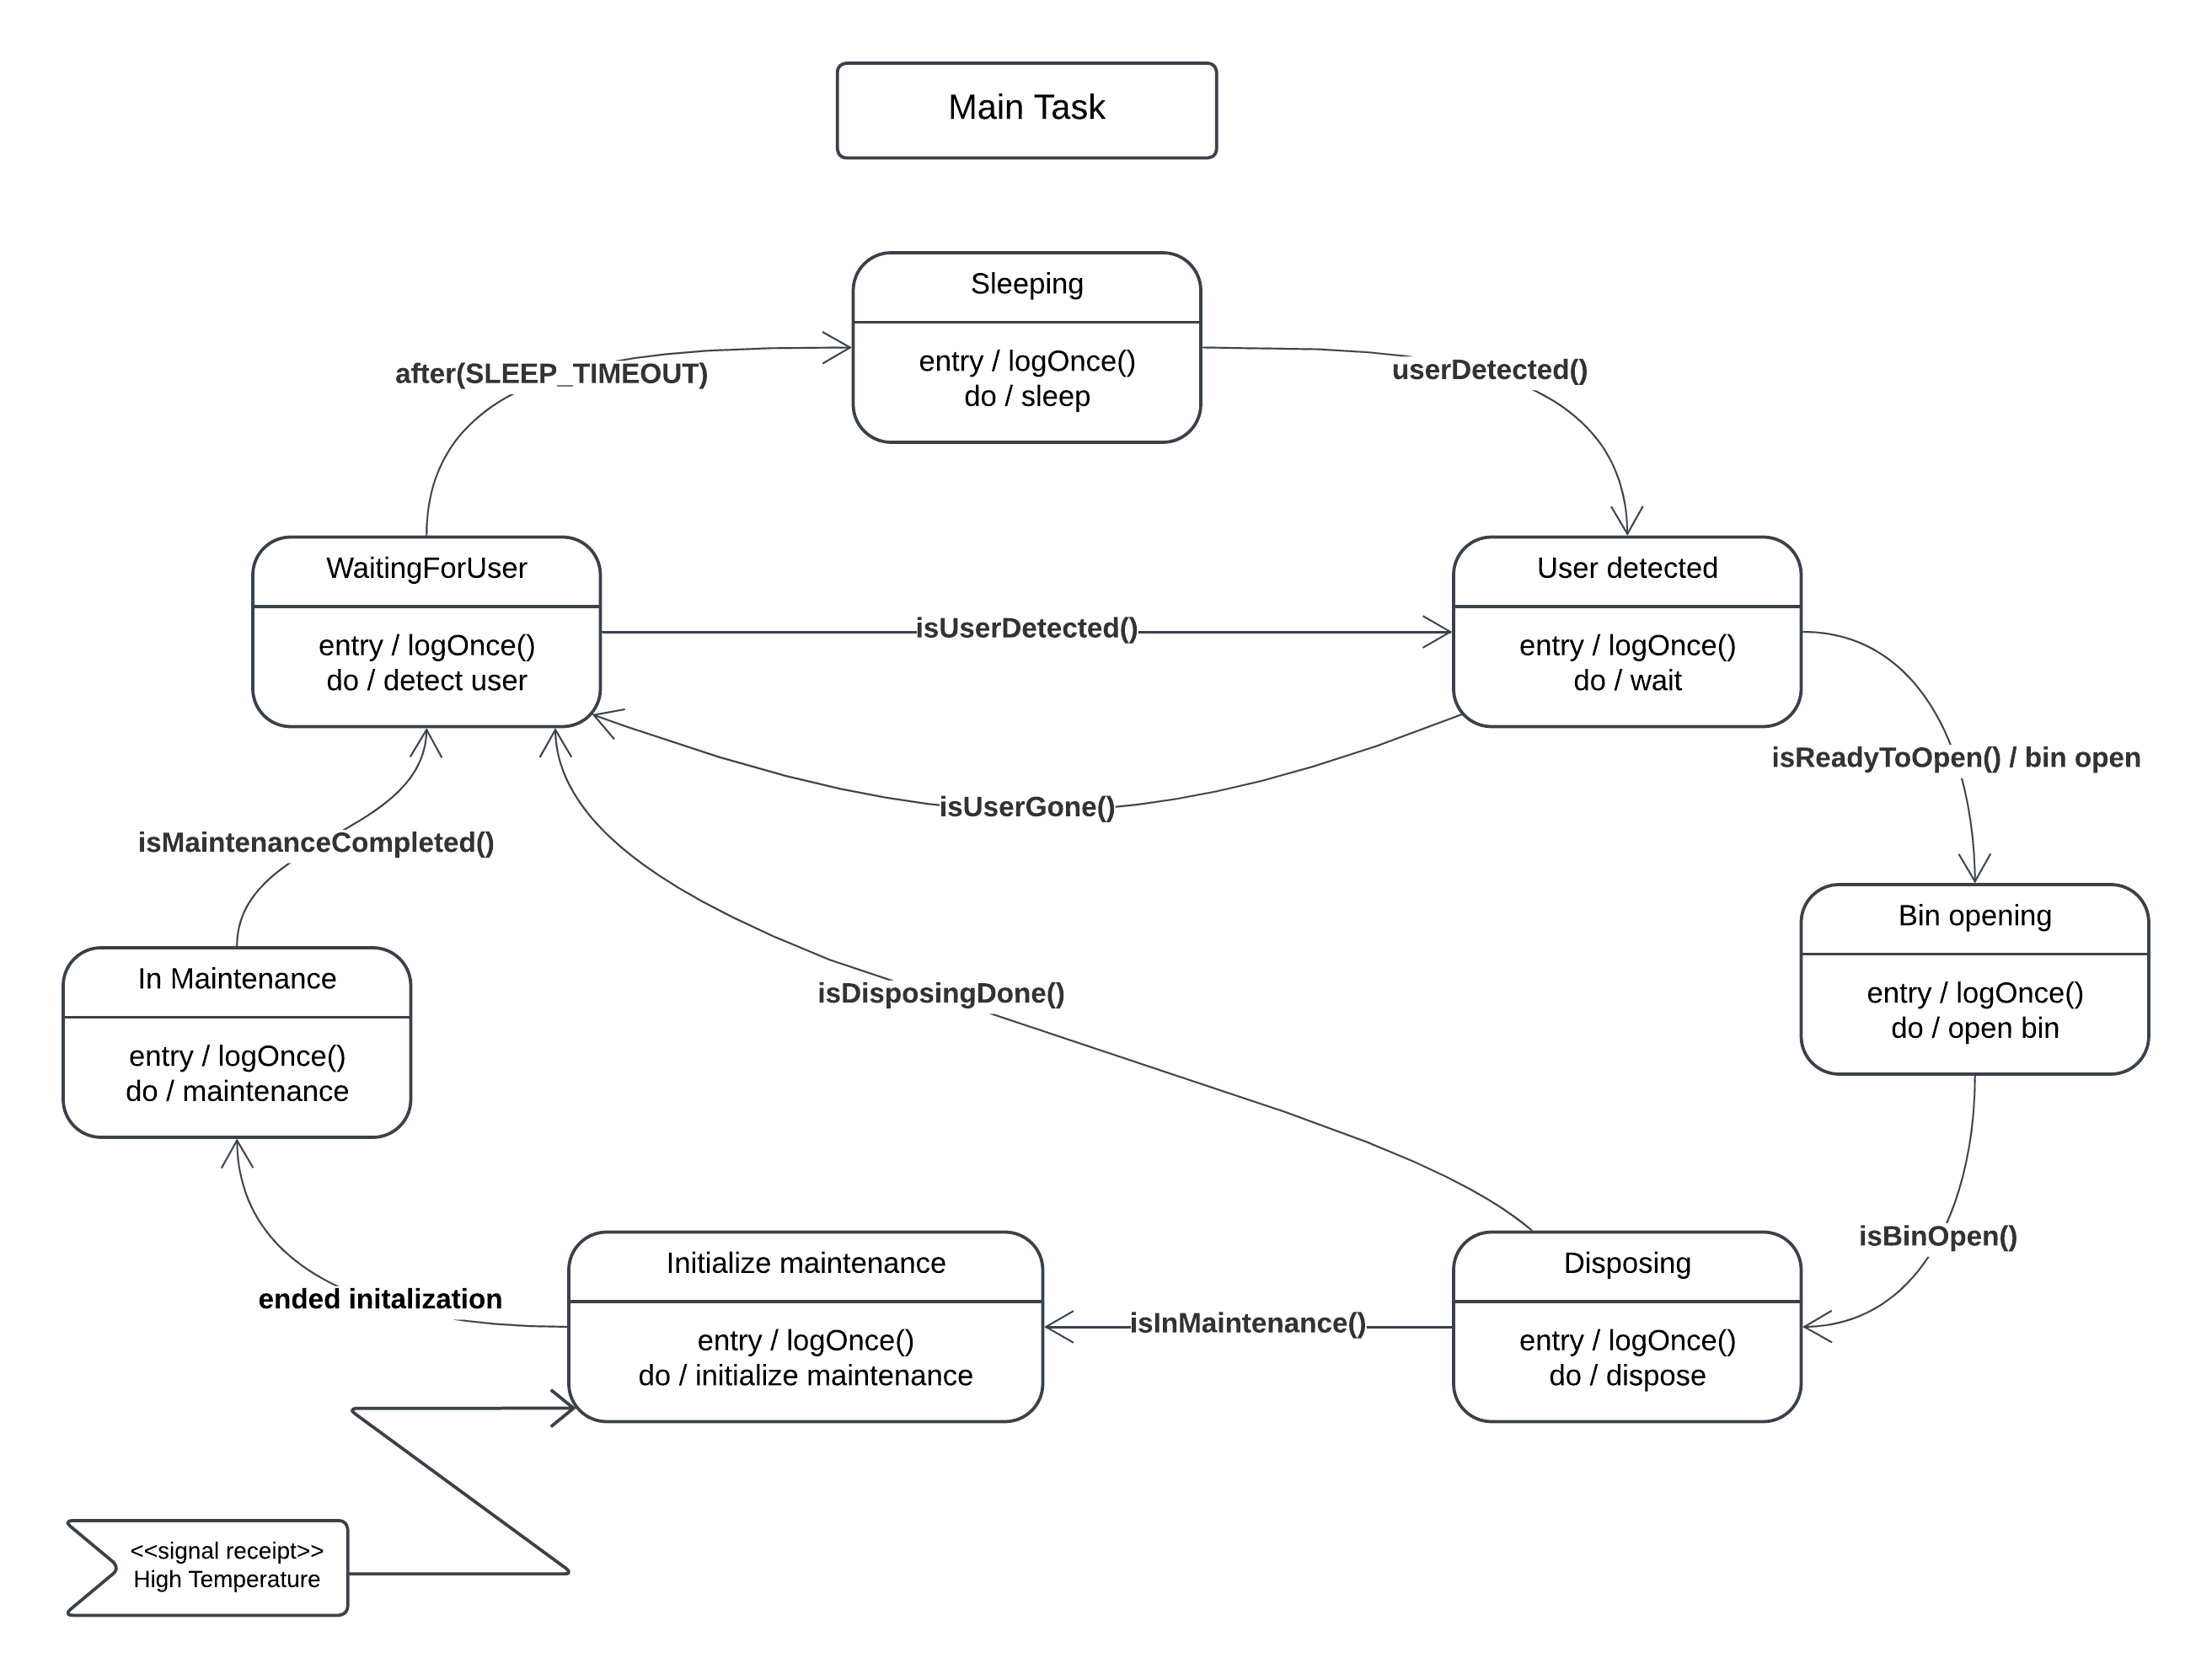
\includegraphics[width=\linewidth]{img/assignment-02/Diagrammi per IOT - MainTask.png}
        \caption{diagramma degli stati di \textit{Main task}}
        \label{fig:main-task}
    \end{figure}
    }
    \item {
    \textbf{User detection task}: effettua la rilevazione della \textbf{presenza dell'utente}. Si occupa di monitorare periodicamente se un utente è vicino al bidone e aggiornare lo stato del sistema di conseguenza.
    \begin{figure}[H]
        \centering
        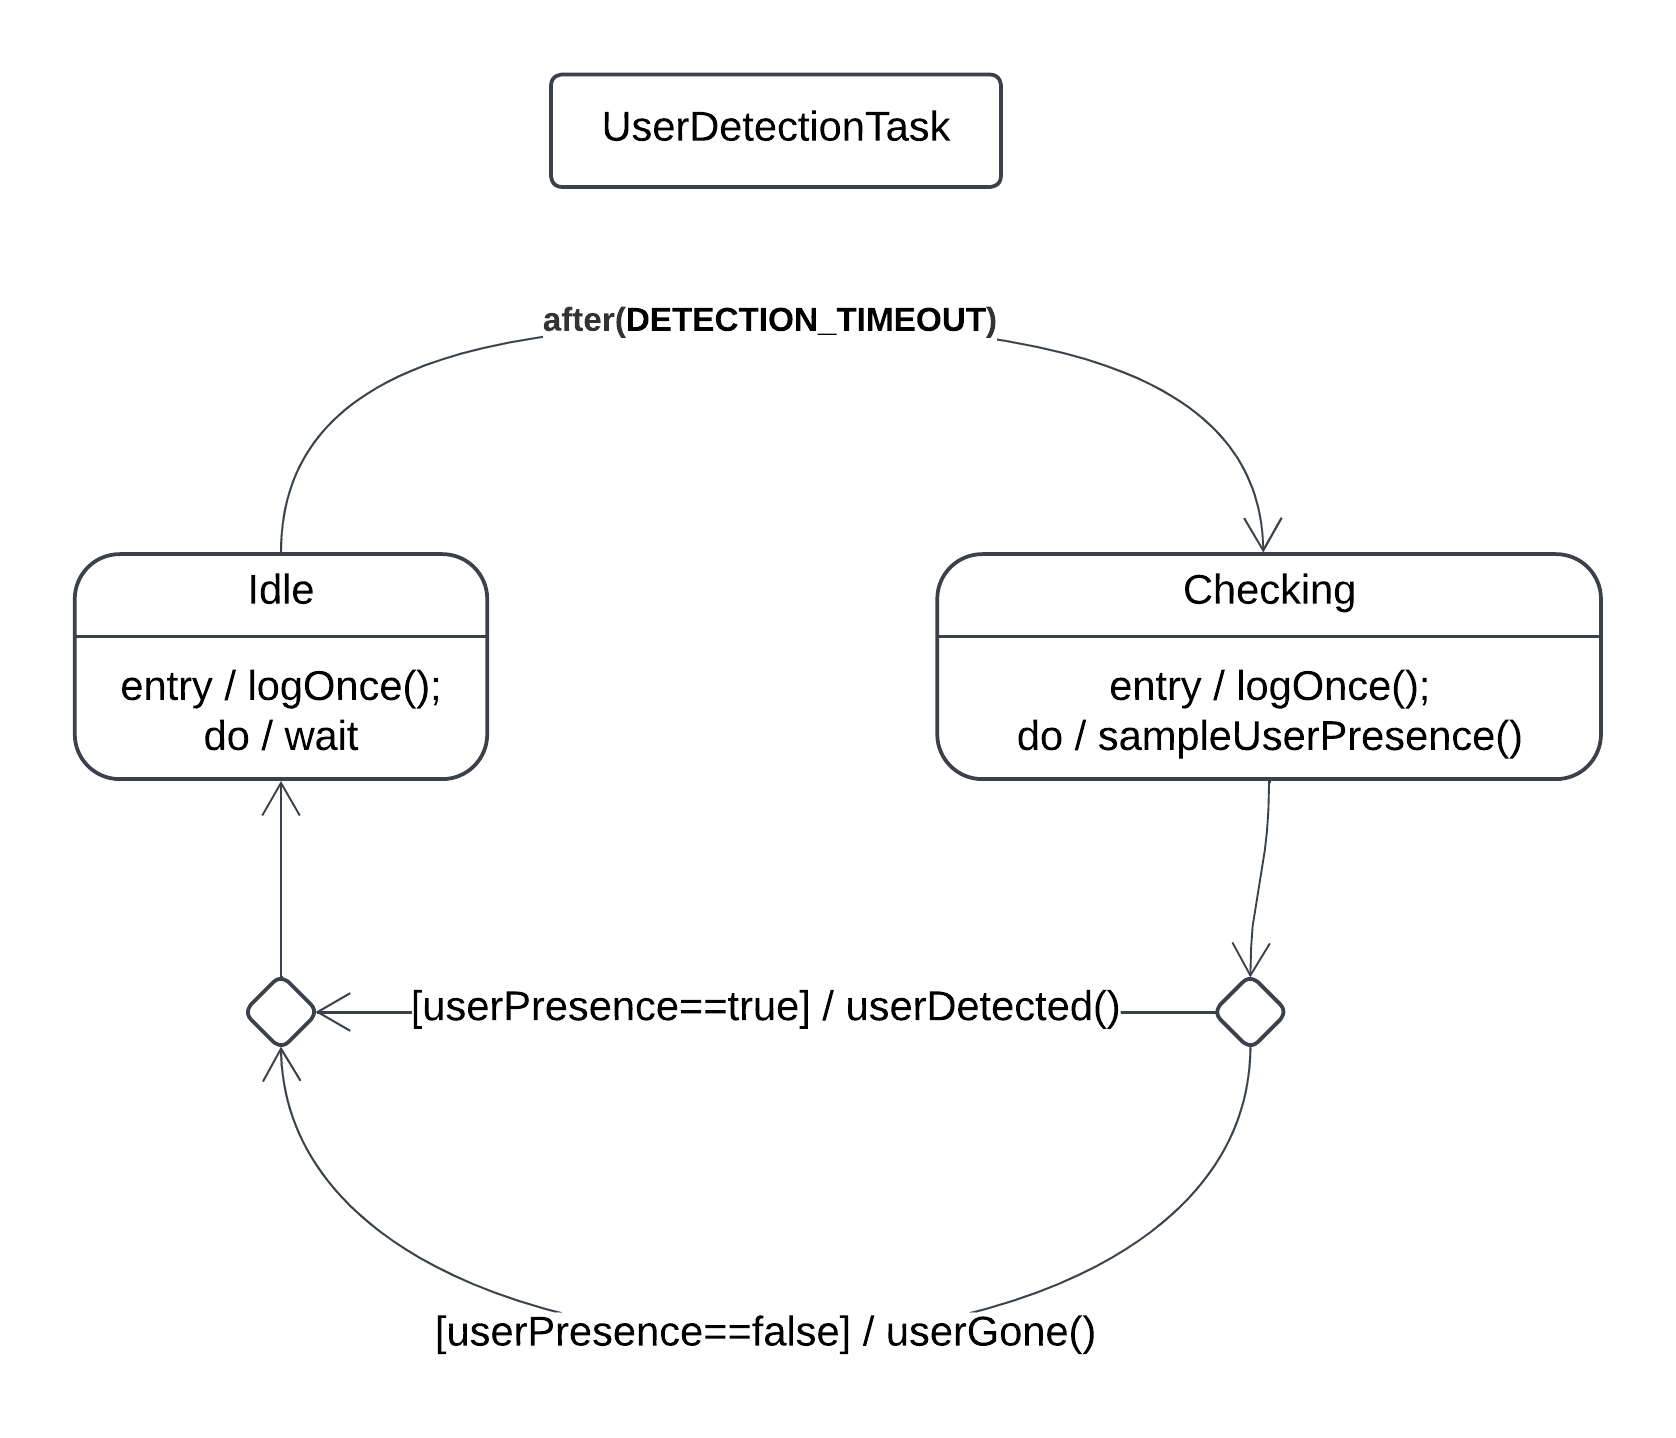
\includegraphics[width=0.7\linewidth]{img/assignment-02/Diagrammi per IOT - User DetectionTask.png}
        \caption{diagramma degli stati di \textit{User detection task}}
        \label{fig:detection-task}
    \end{figure}
    }
    \item {
    \textbf{Maintenance task}: gestisce le operazioni di manutenzione. Si occupa di coordinare le azioni necessarie per la \textbf{manutenzione del sistema} in modo sicuro, come la chiusura del coperchio, la gestione dei messaggi di manutenzione, lo svuotamento del contenitore e il reset dello stato operativo da parte degli operatori.
    \begin{figure}[H]
        \centering
        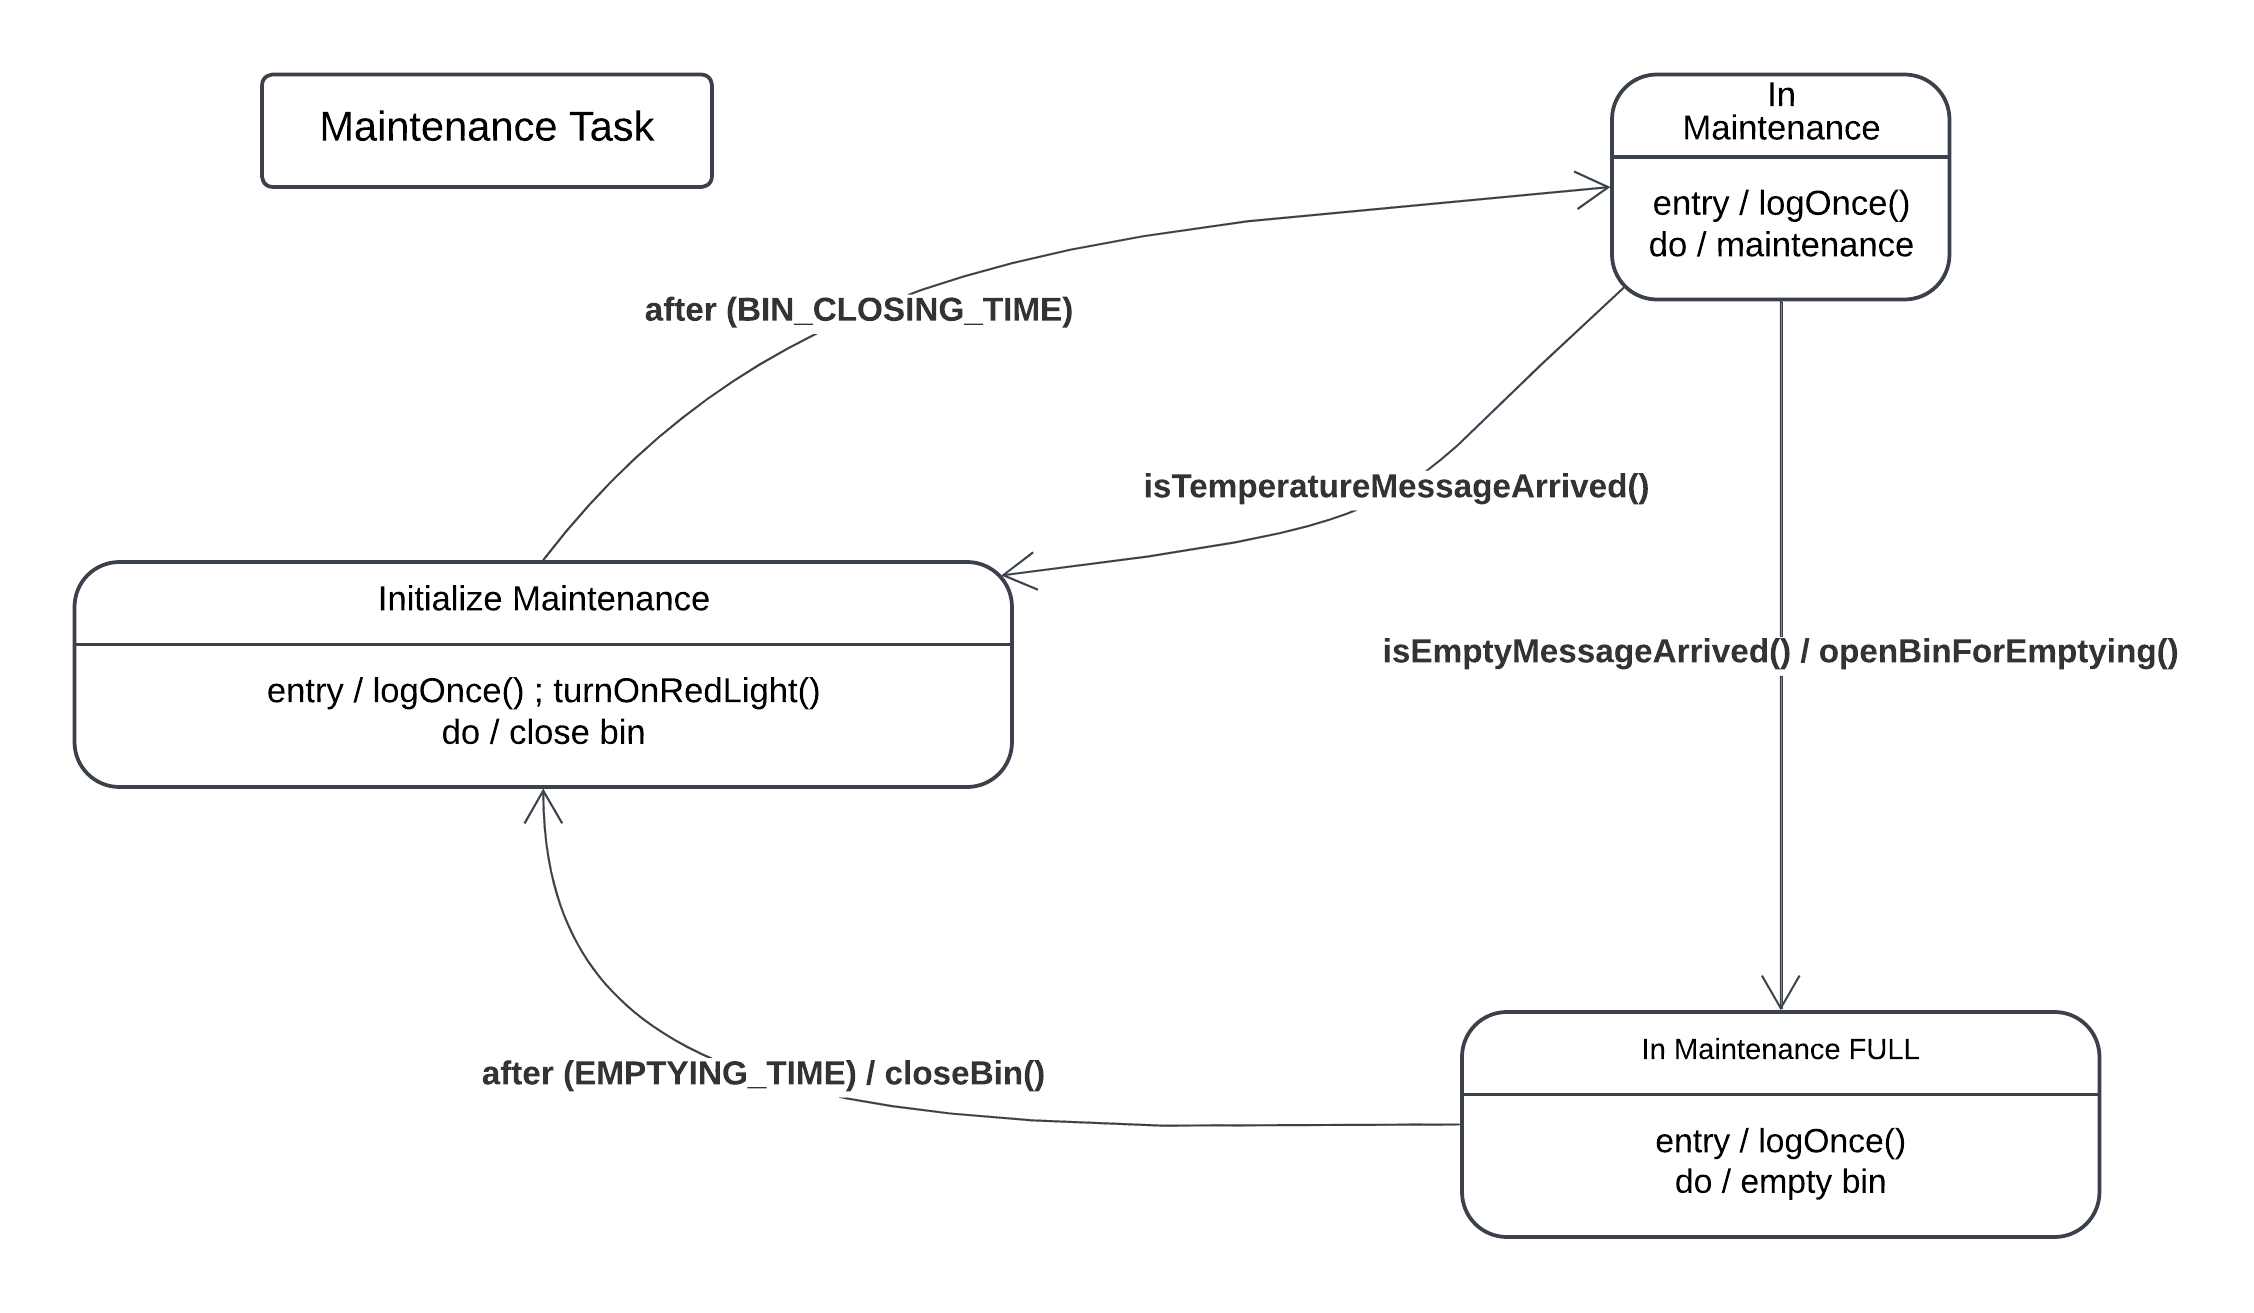
\includegraphics[width=\linewidth]{img/assignment-02/Diagrammi per IOT - MaintenanceTask.png}
        \caption{diagramma degli stati di \textit{Maintenance task}}
        \label{fig:maintenance-task}
    \end{figure}
    }
    \item {
    \textbf{Waste disposal task}: gestisce il \textbf{ciclo di smaltimento dei rifiuti}, coordinando le azioni del bidone dalla fase di apertura fino alla chiusura, verificando anche il riempimento del contenitore rispetto alla soglia critica oltre cui non si può inserire più liquido.
    \begin{figure}[H]
        \centering
        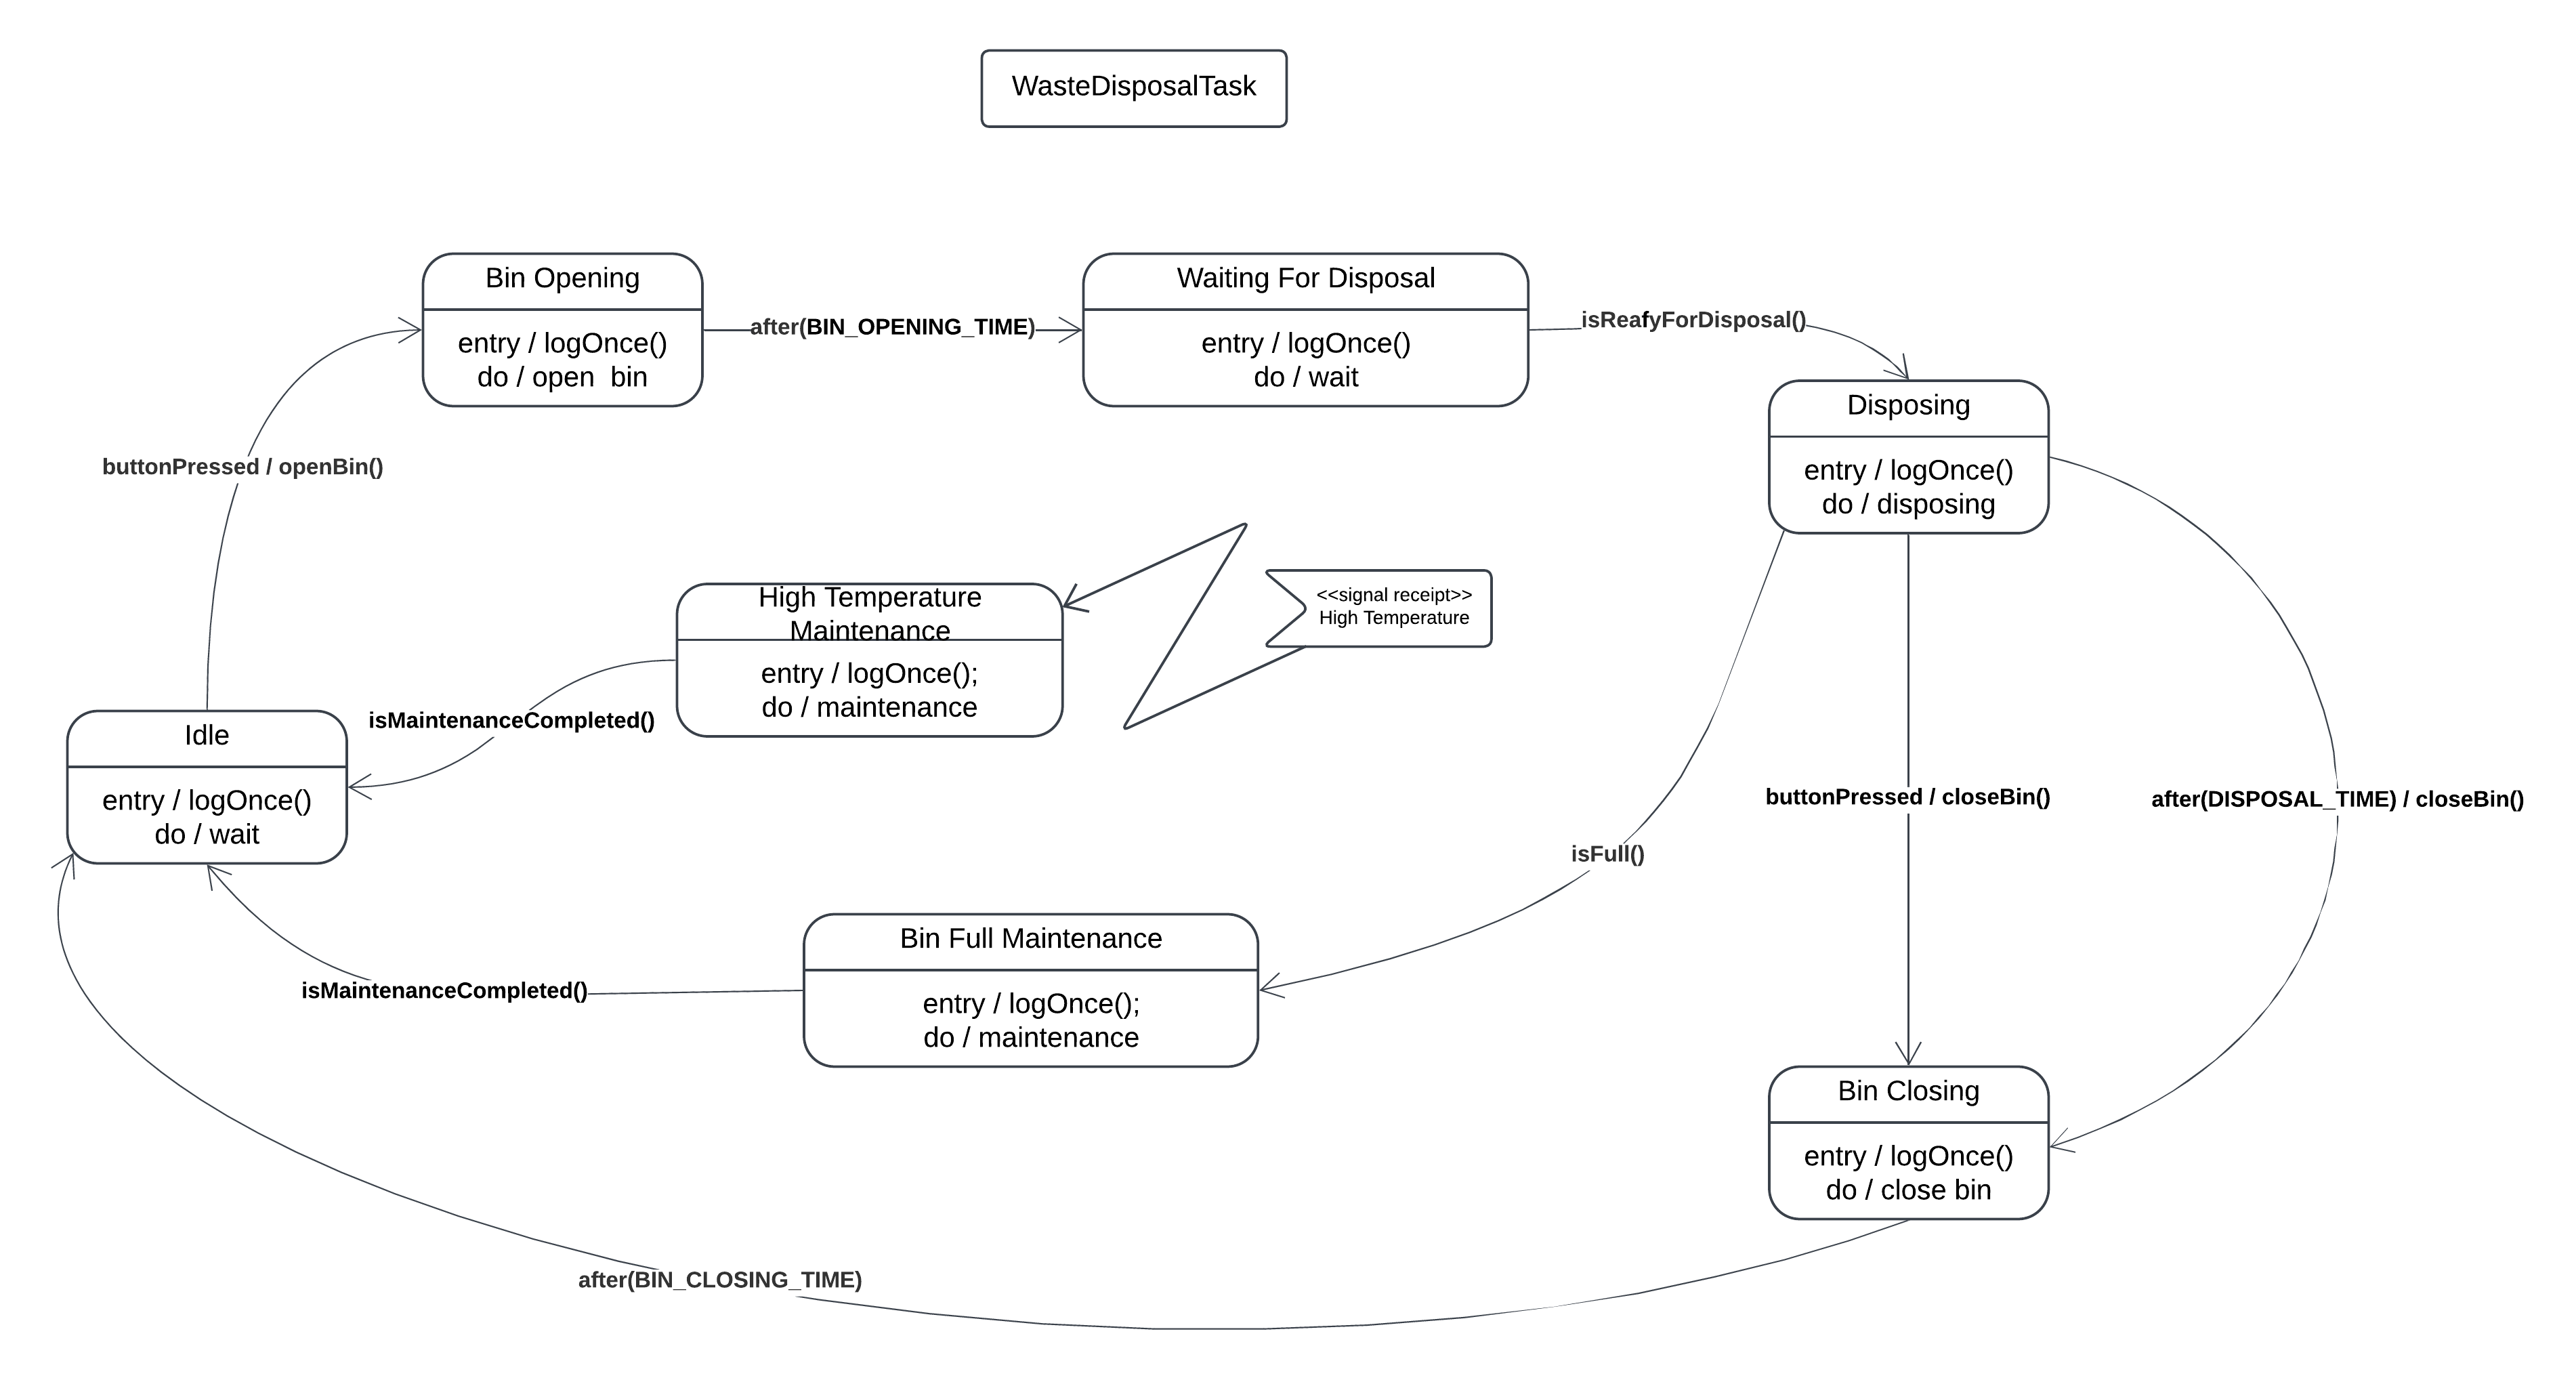
\includegraphics[width=1.2\linewidth]{img/assignment-02/Diagrammi per IOT - WasteDisposalTask.png}
        \caption{diagramma degli stati di \textit{Waste disposal task}}
        \label{fig:waste-task}
    \end{figure}
    }
    \item {
    \textbf{Telemetry task}: è responsabile della \textbf{raccolta e dell'invio periodico dei dati telemetrici} dal sistema verso un applicativo remoto o un servizio di monitoraggio.
    \begin{figure}[H]
        \centering
        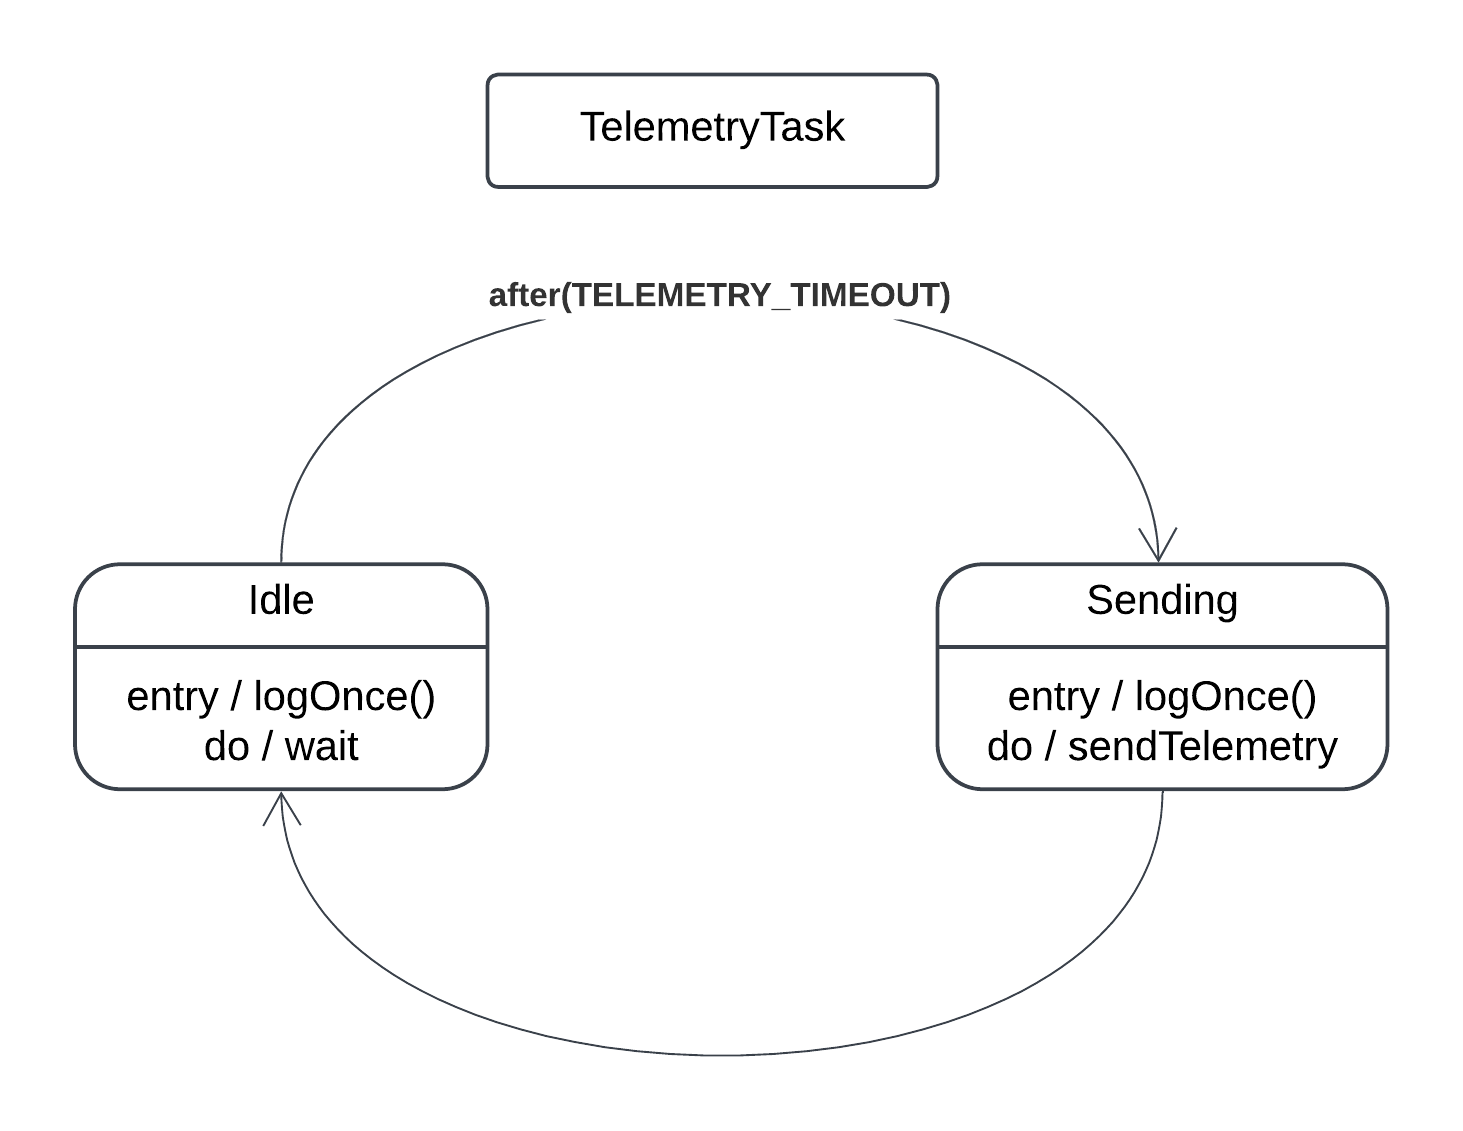
\includegraphics[width=0.6\linewidth]{img/assignment-02/Diagrammi per IOT - Telemetry Task.png}
        \caption{diagramma degli stati di \textit{Telemetry task}}
        \label{fig:telemetry-task}
    \end{figure}
    }
    \item {
    \textbf{Temperature check task}: si occupa di monitorare costantemente la temperatura interna del fluido, per prevenire situazioni pericolose dovute al surriscaldamento ed avvisando gli operatori del raggiungimento della temperatura \textit{critica}.
    \begin{figure}[H]
        \centering
        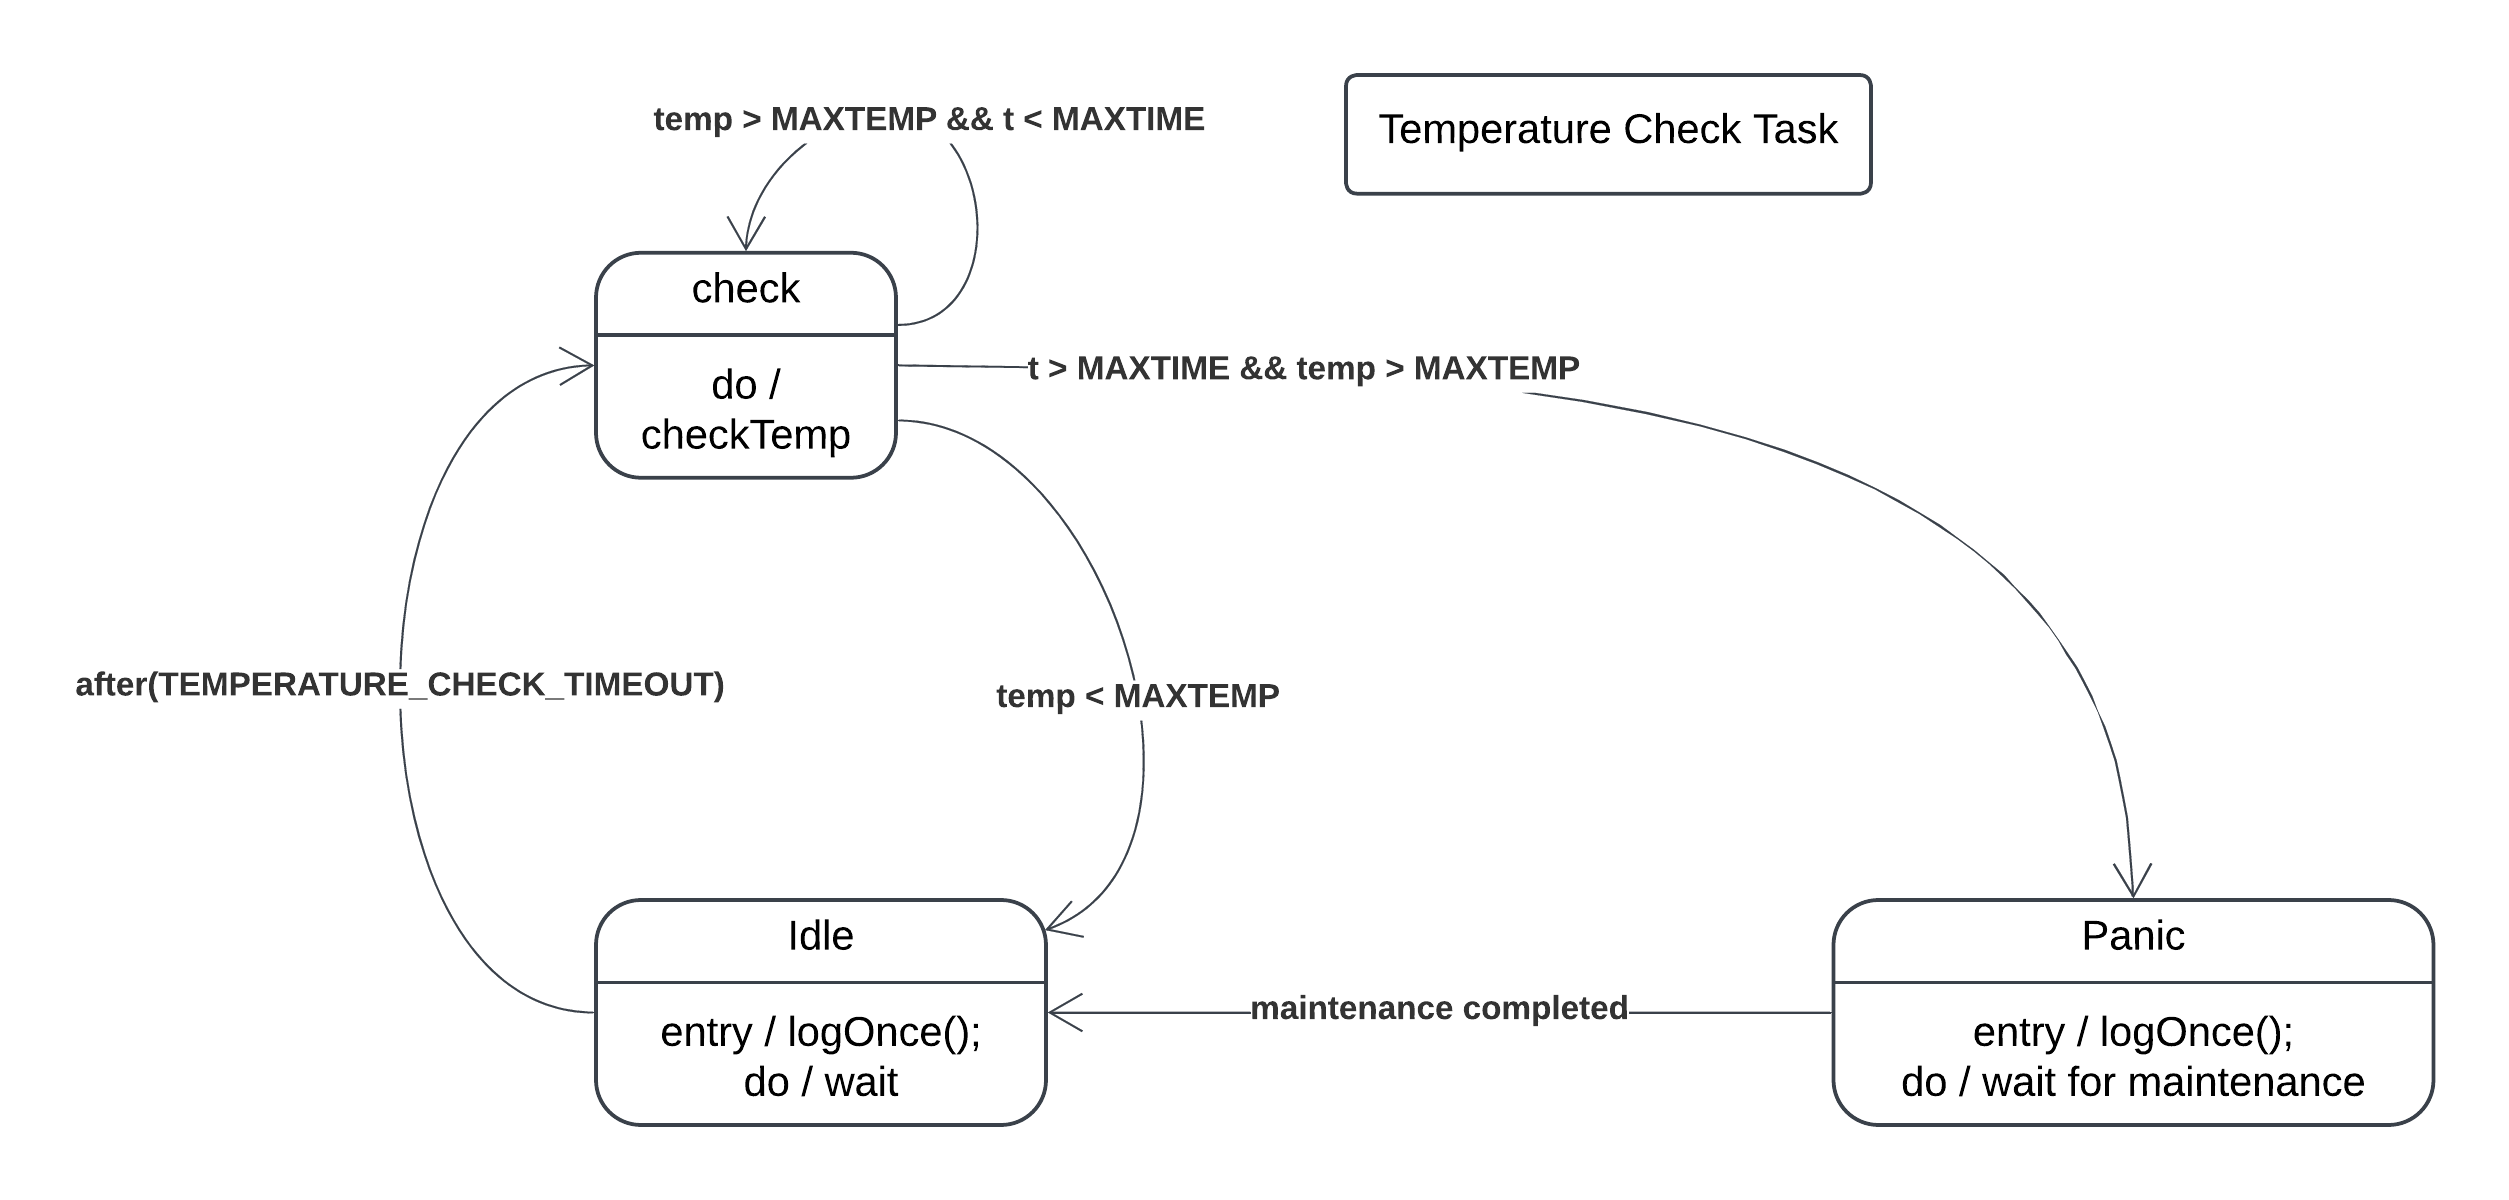
\includegraphics[width=0.9\linewidth]{img/assignment-02/Diagrammi per IOT - Temperature Check Task.png}
        \caption{diagramma degli stati di \textit{Telemetry task}}
        \label{fig:temperature-task}
    \end{figure}
    }
\end{itemize}

\chapter{La Macchina a Stati Finiti}
Come indicato nel capitolo precedente la \hyperref[fig:main-task]{Main task} gestisce il funzionamento dell'intero sistema pertanto può essere presentata come la macchina a stati finiti che lo rappresenta. 

\section{Funzionamento specifico}

\subsection{Rilevamento dell'utente}
\label{sub:utente}
\par {
La macchina a stati finiti (MSF) parte inizialmente nello stato \texttt{WaitingForUser}. Dopo un periodo di inattività, definito SLEEP-TIMEOUT durante il quale non viene rilevata alcuna presenza vicino al bidone, la MSF passa allo stato Sleeping. Quando una persona viene rilevata, il sistema si riattiva e torna nello stato di \texttt{WaitingForUser}.
Quando viene rilevata attività davanti al sensore di movimento la macchina passa nello stato \texttt{UserDetected} ed attende che l'utente interagisca con il pulsante di apertura.
}
\subsection{Inserimento del liquido}
\par {
Se l'utente preme il pulsante di apertura quando il sistema si trova nello stato di User Detected la macchina prima passa allo stato di \texttt{Bin opening} (attendendo che il coperchio si apra) successivamente si passa nello stato \texttt{Disposing}. Successivamente, il bidone si chiuderà in due casi: se l'utente preme il pulsante di chiusura o se scade un tempo limite. Durante la chiusura, il braccio si riporta a 0° (bidone chiuso) e il sistema cambia stato tornando in \texttt{waitingForUser}.\\ \\
\textit{
Tutto questo processo viene fatto in concomitanza con} \hyperref[fig:waste-task]{Waste disposal task} \textit{che coordina anch'essa l'apertura, il tempo di apertura e la chiusura del coperchio (oltre alla rilevazione del livello).
}
}
\subsection{Raggiungimento del livello massimo di liquidi}
\label{sub:liquids}
\par {
Quando la MSF è nello stato \texttt{Disposing}, il sistema può entrare nello stato di \texttt{Initialize maintenance} se il livello di riempimento del contenitore raggiunge o supera una certa soglia. 
\\
\\
\textit{Lo stato di manutenzione è scaturito da } \texttt{Waste disposal task} \textit{ e di conseguenza }\texttt{ Main task e Maintenance Task} \textit{ si attivano per gestire la situazione.}
\\
\\
Il sistema rimane in questo stato finché non riceve un segnale di svuotamento dalla dashboard. Quando il sistema riceve il segnale di svuotamento, il braccio del bidone viene portato a -90° infatti \texttt{Maintenance task} passa allo stato \texttt{In Maintenance FULL}. Il coperchio rimane aperto per un certo tempo dopo il quale \texttt{Maintenance task} termina e viene disattivata, il bidone messo nello stato di quiete e \texttt{Main task} riprende ad attendere utenti come alla sezione \ref{sub:utente}. 
}
\subsection{Superamento della temperatura massima consentita}
\par {
Infine, quando la MSF è in un qualsiasi stato (a parte quello di manutenzione) e la temperatura rilevata dal sensore supera la soglia limite per un periodo definito, il sistema entra immediatamente nello stato \texttt{Initialize maintenance} (analogamente al punto \ref{sub:liquids}).\\
Da questo stato, il sistema può tornare allo stato iniziale solo dopo aver ricevuto un segnale di correzione della temperatura dalla dashboard per poi ritornare nello stato di quiete.
}

\chapter{Circuito}
Di seguito viene riportato lo schema del circuito utilizzato. Si rammenta che potrebbero esserci delle discrepanze tra il circuito realmente realizzato e quello rappresentato in immagine a causa di differenze funzionali nel software di disegno.
\begin{figure}[H]
    \centering
    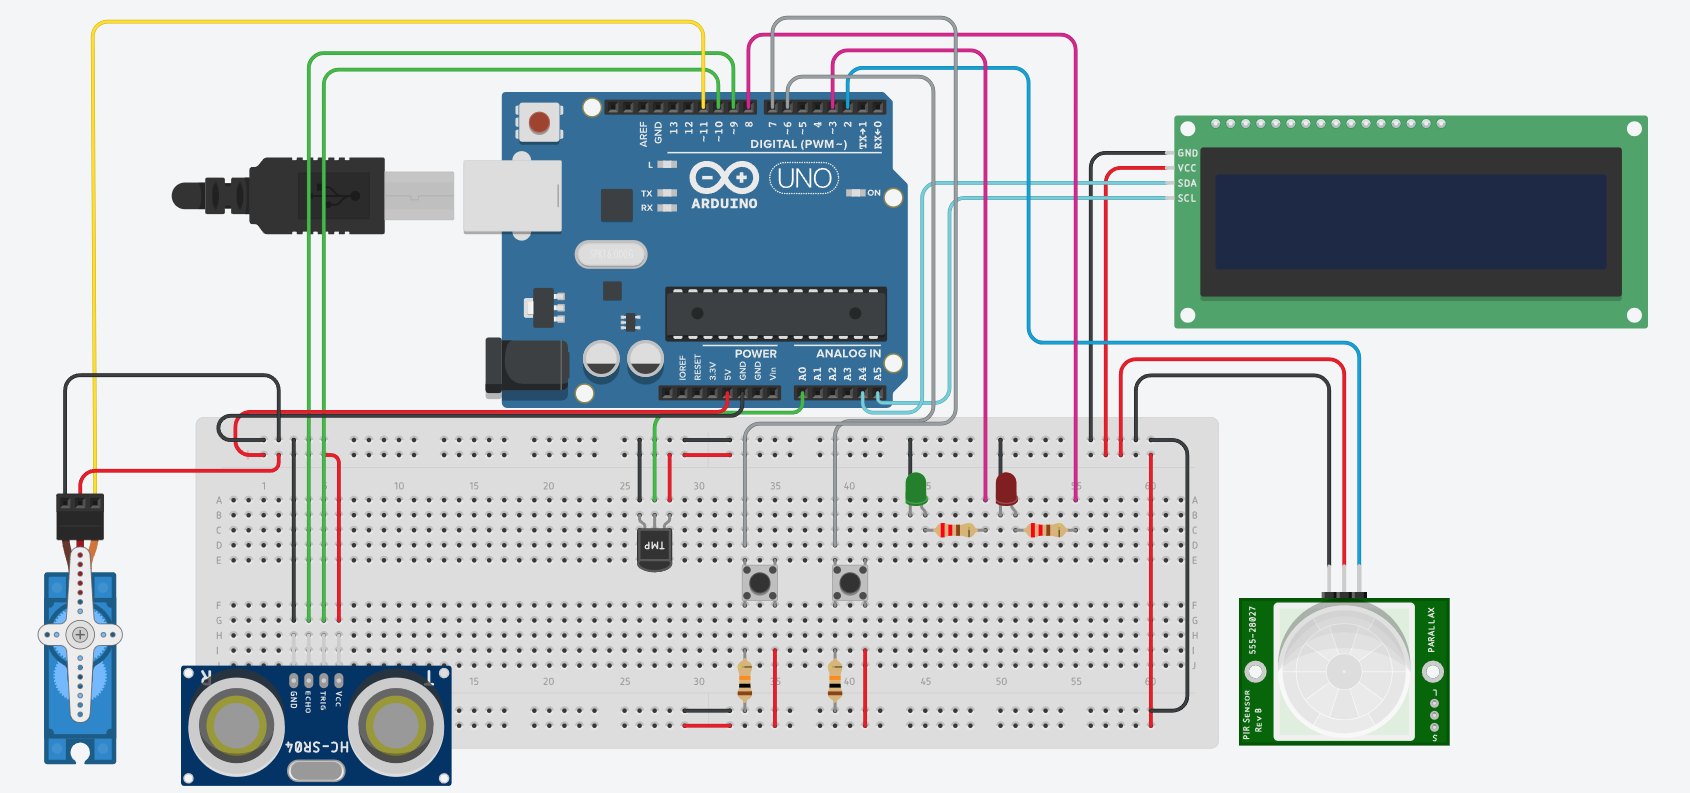
\includegraphics[width=\linewidth]{img/assignment-02/wiring.png}
    \caption{wiring del progetto}
    \label{fig:wiring}
\end{figure}

\end{document}
